\documentclass[11pt,a4paper]{article}

% --- PACKAGES ---
\usepackage[utf8]{inputenc}
\usepackage[margin=1in]{geometry}
\usepackage{amsmath,amssymb,amsfonts}
\usepackage{graphicx,float,booktabs,multirow,array,longtable}
\usepackage{algorithm}
\usepackage{algpseudocode}
\usepackage{hyperref}
\usepackage{titlesec}
\usepackage{enumitem}
\usepackage{caption}
\usepackage{subcaption}
\usepackage{microtype}

% --- NO HEADERS OR FOOTERS ---
\pagestyle{empty}
\let\oldselectfont\selectfont

% --- HYPERREF SETUP (BLACK FONT ONLY, NO COLORED LINKS) ---
\hypersetup{
    hidelinks,
    colorlinks=false,
    pdfborder={0 0 0}
}

% --- SECTION FORMATTING (BLACK FONT ONLY) ---
\titleformat{\section}{\large\bfseries}{\thesection}{1em}{}[\titlerule]
\titleformat{\subsection}{\normalfont\bfseries}{\thesubsection}{1em}{}
\titleformat{\subsubsection}{\normalfont\bfseries}{\thesubsubsection}{1em}{}

\begin{document}
\thispagestyle{empty}

% ==============================================================================
% TITLE PAGE
% ==============================================================================
\begin{titlepage}
    \thispagestyle{empty}
    \centering
    \vspace*{0.8cm}
    
    {\Huge \bfseries Dynamic Emergency Resource Allocation via Deep Reinforcement Learning \par}
    \vspace{0.4cm}
    {\LARGE \itshape A Data-Driven Framework for Urban Emergency Medical Services Dispatching \par}
    
    \vspace{1.0cm}
    \rule{\linewidth}{1pt}
    \vspace{0.8cm}
    
    % --- AUTHORS ---
    \begin{minipage}{0.48\textwidth}
        \begin{center} \large
            \textbf{Parimisetty Sneha Deepika}\\
            AV.SC.U4AIE23034\\
            Amrita Vishwa Vidyapeetham
        \end{center}
    \end{minipage}
    \hfill
    \begin{minipage}{0.48\textwidth}
        \begin{center} \large
            \textbf{Nakka Keerthi}\\
            AV.SC.U4AIE23032\\
            Amrita Vishwa Vidyapeetham
        \end{center}
    \end{minipage}
    
    \vspace{1.0cm}
    
    % --- COURSE & DATASET DETAILS ---
    \begin{center}
        \large
        \textbf{Course Name:} Reinforcement Learning \quad | \quad \textbf{Course Code:} [Course Code] \\
        \textbf{Course Instructor:} [Instructor Name] \\
        \textbf{Dataset Used:} NYC EMS Dispatch Data (274,964 Records), NYS Hospital Capacity \& US Census ZCTA
    \end{center}
    
    \vspace{0.8cm}
    
    % --- ABSTRACT ---
    \begin{abstract}
    \noindent Urban Emergency Medical Services (EMS) face constant pressure from shifting dispatch demand, traffic bottlenecks, and sudden surges in hospital bed utilization. Traditional dispatch systems rely heavily on simple proximity rules—sending an ambulance to whichever hospital is physically closest. While this keeps initial driving distances low, it often causes localized hospital crowding, forces ambulances to wait in long admission queues, and leaves regional medical resources poorly balanced. This report presents a dynamic reinforcement learning framework designed to route emergency patients across urban hospital networks in real time. We built a custom simulation environment using 274,964 clean EMS dispatch records from New York City, combined with OpenStreetMap driving networks and actual bed capacity data from New York State hospitals. We evaluated a Deep Q-Network (DQN) model against several practical dispatch strategies, including Nearest Hospital, Weighted Heuristic, Capacity-First, and Random allocation. Our tests look closely at average transport times, critical patient safety, hospital load balancing using Jain's Fairness Index, multi-seed stability, and stress scenarios such as bed shortages and demand spikes. The results show that while nearest-hospital routing gives the shortest travel times under light traffic (around 12.1 minutes), the trained DQN model balances transport distance with hospital capacity, preventing facility overloads and keeping dispatch performance steady even when hospital capacities drop.
    \end{abstract}
    
    \vspace{0.4cm}
    
    {\small \textbf{Keywords:} Deep Reinforcement Learning, Deep Q-Networks, Emergency Medical Services, Urban Resource Allocation, Hospital Bed Capacity, Dynamic Routing, Jain's Fairness Index.}
    
\end{titlepage}

\newpage
\thispagestyle{empty}
\tableofcontents
\newpage
\thispagestyle{empty}

% ==============================================================================
% SECTION 1: INTRODUCTION AND PROBLEM STATEMENT
% ==============================================================================
\section{Introduction and Problem Statement}
\label{sec:intro}

\subsection{Motivation and Real-World Context}
Managing emergency medical services in a dense city like New York is an enormous operational challenge. Every day, dispatchers handle thousands of calls ranging from life-threatening cardiac arrests and major trauma to minor injuries and non-urgent patient transfers. The primary goal of an EMS system is simple: get the patient to an appropriate hospital as fast as possible without overwhelming any single facility.

In practice, most municipal dispatch centers rely on static proximity rules. When an ambulance crew finishes stabilizing a patient on scene, they default to driving to the nearest hospital. While this approach seems logical on paper, it creates several practical problems in real-world urban operations:
\begin{itemize}[leftmargin=*]
    \item \textbf{Hospital Overcrowding:} If multiple emergencies happen near the same neighborhood, all ambulances head to the exact same emergency room. That facility gets bottlenecked while another hospital ten minutes away sits half-empty.
    \item \textbf{Ambulance Wall Time:} When an emergency room gets overloaded, incoming ambulances must wait outside with their patients until a bed opens up. This keeps ambulances off the road and unavailable for new incoming calls.
    \item \textbf{Vulnerability to Surges:} During extreme events—such as bad winter storms, major traffic accidents, or disease outbreaks—static nearest-hospital routing fails quickly because key trauma centers fill up almost immediately.
\end{itemize}

\subsection{Problem Statement}
This project investigates whether dynamic, data-driven decision-making can improve how patients are allocated across hospitals. Specifically, we focus on answering a practical question:

\begin{quote}
\textit{Can a Deep Q-Network (DQN) policy route emergency patients across a city's hospital network more effectively than standard proximity rules, balancing fast transport times with hospital bed availability?}
\end{quote}

\subsection{Key Contributions}
The main contributions of this work are:
\begin{enumerate}[leftmargin=*]
    \item \textbf{Real Dataset Integration:} We curated 274,964 clean EMS dispatch records from NYC Open Data, matched them to 229 ZIP Code spatial centroids, and integrated actual hospital bed capacities from the New York State Department of Health.
    \item \textbf{Realistic Simulation Environment:} We constructed a Gymnasium-compliant simulation that tracks real road distances via OpenStreetMap, models time-of-day demand shifts, and simulates dynamic patient discharge queues based on case severity.
    \item \textbf{Direct Policy Comparison:} We benchmarked the trained DQN agent against four traditional rules (Nearest, Weighted Heuristic, Capacity-First, and Random) across normal operation, critical medical cases, multi-seed statistical runs, and stress scenarios.
    \item \textbf{Fairness Evaluation:} We measured how evenly each policy distributes patient volume across hospitals using Jain's Fairness Index.
\end{enumerate}

% ==============================================================================
% SECTION 2: BACKGROUND THEORY
% ==============================================================================
\section{Background Theory}
\label{sec:background}

\subsection{Emergency Routing and Spatial Distance}
To estimate travel time between an emergency location and a candidate hospital, we need a realistic representation of urban road distances. In our framework, emergency call locations are grouped by ZIP code centroids $(lat_z, lon_z)$, and hospitals are located at coordinates $(lat_h, lon_h)$. 

We calculate road transport time using a straightforward relationship:
\begin{equation}
    \text{Travel Time (minutes)} = \frac{\text{Distance (km)}}{\text{Average EMS Speed (km/h)}} \times 60
\end{equation}
Where average EMS travel speed is set to an empirical urban benchmark of 28 km/h. Distance is computed either using OpenStreetMap road network graphs via Dijkstra's shortest path algorithm or using Haversine distance scaled by a standard urban road circuity factor of 1.35.

\subsection{Markov Decision Processes}
We model the emergency dispatch problem as a Markov Decision Process (MDP). At each step, an incident occurs, and the system must choose which hospital should receive the patient:
\begin{itemize}[leftmargin=*]
    \item \textbf{State Space:} Captures the call location, case severity, time of day, current hourly demand, and current bed occupancy levels across all regional hospitals.
    \item \textbf{Action Space:} The choice of destination hospital from the available regional network.
    \item \textbf{Transitions:} When a patient is sent to a hospital, that hospital's occupancy increases. Over time, admitted patients complete their care and are discharged, freeing up beds.
    \item \textbf{Reward Function:} A scalar score that penalizes travel time and high hospital occupancy while rewarding successful admissions.
\end{itemize}

\subsection{Deep Q-Learning}
Because the state representation includes continuous hospital occupancy levels and hundreds of spatial zones, simple lookup tables are not feasible. We use a Deep Q-Network (DQN) to approximate the value of choosing each hospital given the current state. The network takes the state vector as input and outputs expected long-term rewards for each hospital choice.

To keep training stable, the DQN uses two standard techniques:
\begin{enumerate}[leftmargin=*]
    \item \textbf{Replay Buffer:} Past experiences are saved in a memory buffer. During training, random mini-batches are sampled from this buffer to prevent consecutive steps from confusing the neural network.
    \item \textbf{Target Network:} A copy of the Q-network is kept frozen and updated only periodically. This stops the target values from changing continuously while the model updates its weights.
\end{enumerate}

\subsection{Jain's Fairness Index}
To measure how fairly patient load is distributed among hospitals, we use Jain's Fairness Index:
\begin{equation}
    J = \frac{\left( \sum_{i=1}^{N} x_i \right)^2}{N \cdot \sum_{i=1}^{N} x_i^2}
\end{equation}
Here, $x_i$ represents the final occupancy fraction of hospital $i$, and $N$ is the total number of hospitals. A score of 1.0 means every hospital is used equally, while lower scores show that a few hospitals are taking on most of the load.

% ==============================================================================
% SECTION 3: METHODOLOGY AND IMPLEMENTATION DETAILS
% ==============================================================================
\section{Methodology and Implementation Details}
\label{sec:methodology}

\subsection{Data Pipeline and Cleaning}
Our dataset is built from three sources:
\begin{enumerate}[leftmargin=*]
    \item \textbf{NYC EMS Incident Records:} 300,000 raw incidents collected between October and December 2025. After filtering out invalid coordinates and bad timestamps, we retained 274,964 clean records.
    \item \textbf{US Census ZCTA Gazetteer:} Provides geographical centroids for 229 ZIP code zones in NYC.
    \item \textbf{NYS Department of Health Records:} Provides operational capacities for 12 major healthcare facilities across Manhattan, Queens, Brooklyn, and the Bronx.
\end{enumerate}

\begin{table}[H]
    \centering
    \caption{Key Characteristics of the Processed EMS Dataset.}
    \label{tab:ems_summary}
    \resizebox{\columnwidth}{!}{%
    \begin{tabular}{ll}
        \toprule
        \textbf{Metric / Feature} & \textbf{Value / Details} \\
        \midrule
        Raw Incident Count & 300,000 \\
        Clean Processed Incidents & 274,964 \\
        Unique Spatial Demand Zones & 229 ZIP Code Areas \\
        Destination Healthcare Facilities & 12 NYC Hospitals \\
        Median Empirical Travel Time & 8.53 minutes \\
        Critical Severity Calls (Severity 0) & 24.51\% (Stay: 5--14 steps) \\
        Moderate Severity Calls (Severity 1) & 52.79\% (Stay: 4--11 steps) \\
        Low Severity Calls (Severity 2) & 22.70\% (Stay: 2--8 steps) \\
        Assumed Average EMS Speed & 28.0 km/h \\
        \bottomrule
    \end{tabular}%
    }
\end{table}

\subsection{State Representation and Environment Setup}
The environment observation vector has 258 features:
\begin{itemize}[leftmargin=*]
    \item \textbf{Spatial Zone (229 values):} A one-hot vector indicating which ZIP code zone the incident occurred in.
    \item \textbf{Context Features (5 values):} Patient severity (0 for critical, 1 for moderate, 2 for low), sine/cosine encodings for hour of day, a weekend flag, and current hourly call volume.
    \item \textbf{Hospital Occupancy (12 values):} Current occupied bed fraction for each hospital.
    \item \textbf{Hospital Free Capacity (12 values):} Remaining available bed fraction for each hospital.
\end{itemize}

\subsection{Dynamic Discharge Queues}
Patients do not vanish immediately after admission. The simulation tracks patient stays using discrete timers. Depending on case severity, each admitted patient stays in the hospital queue for a sampled number of simulation steps:
\begin{itemize}[leftmargin=*]
    \item \textbf{Critical (Severity 0):} Uniform random stay between 5 and 14 steps.
    \item \textbf{Moderate (Severity 1):} Uniform random stay between 4 and 11 steps.
    \item \textbf{Low (Severity 2):} Uniform random stay between 2 and 8 steps.
\end{itemize}
At each step, remaining stay timers count down by one. When a timer hits zero, the patient is discharged and bed space is freed up.

\subsection{Reward Function}
The reward function balances travel speed against hospital load:
\begin{equation}
    \text{Reward} = -1.0 \times \left(\frac{\text{Travel Min}}{10}\right) - 4.0 \times (\text{Occupancy})^2 + 5.0 \, [\text{if admitted}]
\end{equation}
If an ambulance selects a hospital that is at 100\% capacity, a heavy penalty (-30.0) is applied. Additionally, if a critical patient (Severity 0) is sent to a hospital that is already over 85\% full, an extra penalty (-10.0) is triggered.

\subsection{Algorithms}
Algorithm \ref{alg:env_step} outlines the environment step function, and Algorithm \ref{alg:dqn_train} shows the training loop for the DQN model.

\begin{algorithm}[H]
\caption{Environment Step and Dynamic Queue Update}
\label{alg:env_step}
\begin{algorithmic}[1]
\State \textbf{Input:} Action $a$ (chosen hospital index)
\State Update stay timers in all hospital queues; discharge completed patients
\State Calculate travel time $T$ from call zone to hospital $a$
\If{Hospital $a$ has an open bed}
    \State Add patient to Hospital $a$ queue with sampled stay duration
    \State $\text{Reward} \leftarrow -1.0 \times (T / 10.0) - 4.0 \times (\text{Occupancy}_a)^2 + 5.0$
    \If{Severity is Critical \textbf{and} $\text{Occupancy}_a > 0.85$}
        \State $\text{Reward} \leftarrow \text{Reward} - 10.0$
    \EndIf
\Else
    \State $\text{Reward} \leftarrow -30.0 - 1.0 \times (T / 10.0)$
\EndIf
\State Advance event pointer and return next state, reward, and status flags
\end{algorithmic}
\end{algorithm}

\begin{algorithm}[H]
\caption{DQN Policy Training Loop}
\label{alg:dqn_train}
\begin{algorithmic}[1]
\State Initialize replay buffer $\mathcal{D}$ (capacity 50,000) and Q-network weights
\For{episode $= 1 \dots E$}
    \State Reset environment and get initial state $s_0$
    \For{step $t = 0 \dots T_{\text{max}}-1$}
        \State Select action $a_t$ using $\epsilon$-greedy rule
        \State Execute $a_t$, observe reward $r_t$ and next state $s_{t+1}$
        \State Store transition $(s_t, a_t, r_t, s_{t+1})$ in buffer $\mathcal{D}$
        \If{Buffer has enough samples}
            \State Sample mini-batch of 64 transitions and update Q-network weights
        \EndIf
        \State Periodically update target network weights
    \EndFor
\EndFor
\end{algorithmic}
\end{algorithm}

% ==============================================================================
% SECTION 4: EXPERIMENTAL SETUP
% ==============================================================================
\section{Experimental Setup}
\label{sec:experiments}

\subsection{Data Splitting}
We split the 274,964 clean EMS calls chronologically to keep the test evaluation clean:
\begin{itemize}[leftmargin=*]
    \item \textbf{Train Set (70\%):} 192,475 calls for model training.
    \item \textbf{Validation Set (15\%):} 41,245 calls for parameter tuning.
    \item \textbf{Test Set (15\%):} 41,244 calls for final policy testing.
\end{itemize}

\subsection{Compared Policies}
We benchmarked five different dispatch policies:
\begin{enumerate}[leftmargin=*]
    \item \textbf{Nearest:} Sends the ambulance to the closest hospital with an available bed.
    \item \textbf{Weighted Heuristic:} Scores hospitals using a combination of travel distance and current occupancy. Critical cases weight distance higher (0.75 distance / 0.25 occupancy), while minor cases balance them more evenly (0.55 distance / 0.45 occupancy).
    \item \textbf{DQN:} The trained deep reinforcement learning model.
    \item \textbf{Capacity-First:} Sends the patient to whichever hospital currently has the highest percentage of free beds.
    \item \textbf{Random:} Selects randomly among hospitals that have open beds.
\end{enumerate}

\subsection{Model Hyperparameters}
Table \ref{tab:hyperparams} lists the main settings used to train the DQN agent.

\begin{table}[H]
    \centering
    \caption{DQN Training Hyperparameters.}
    \label{tab:hyperparams}
    \resizebox{\columnwidth}{!}{%
    \begin{tabular}{ll}
        \toprule
        \textbf{Parameter} & \textbf{Setting} \\
        \midrule
        Neural Architecture & 2 Hidden Layers $\times$ 256 Units \\
        Activation Function & ReLU \\
        Optimizer & Adam (learning rate = $10^{-4}$) \\
        Discount Factor ($\gamma$) & 0.98 \\
        Replay Buffer Capacity & 50,000 steps \\
        Batch Size & 64 \\
        Exploration ($\epsilon$) & Decays from 1.0 to 0.05 over 12,500 steps \\
        Total Training Steps & 50,000 steps \\
        \bottomrule
    \end{tabular}%
    }
\end{table}

\subsection{Stress Scenarios}
We tested all policies across four operational conditions:
\begin{itemize}[leftmargin=*]
    \item \textbf{Normal:} Standard starting occupancy (25\% to 55\%).
    \item \textbf{High Congestion:} Elevated starting occupancy (55\% to 85\%).
    \item \textbf{Critical Shortage:} Near-capacity starting occupancy (75\% to 95\%).
    \item \textbf{Demand Surge:} Standard occupancy with a 1.75$\times$ multiplier on incoming call rate.
\end{itemize}

% ==============================================================================
% SECTION 5: RESULTS AND ANALYSIS
% ==============================================================================
\section{Results and Analysis}
\label{sec:results}

\subsection{Standard Policy Evaluation}
Table \ref{tab:normal_results} shows performance across 80 evaluation episodes under normal conditions.

\begin{table}[H]
    \centering
    \caption{Policy Performance Comparison under Normal Conditions.}
    \label{tab:normal_results}
    \resizebox{\columnwidth}{!}{%
    \begin{tabular}{lccccc}
        \toprule
        \textbf{Policy} & \textbf{Mean Reward} & \textbf{Travel Time (min)} & \textbf{Overload Rate} & \textbf{Success Rate} & \textbf{Mean Util.} \\
        \midrule
        \textbf{Nearest} & \textbf{3.7606} & \textbf{12.14} & 0.00\% & 100.0\% & 2.79\% \\
        \textbf{WeightedHeuristic} & 3.7592 & 12.21 & 0.00\% & 100.0\% & 2.52\% \\
        \textbf{DQN} & 3.2712 & 17.04 & 0.00\% & 100.0\% & 2.86\% \\
        \textbf{CapacityFirst} & 1.1838 & 38.05 & 0.00\% & 100.0\% & 1.75\% \\
        \textbf{Random} & 1.0624 & 39.13 & 0.00\% & 100.0\% & 2.70\% \\
        \bottomrule
    \end{tabular}%
    }
\end{table}

Figure \ref{fig:travel_time_plot} displays the average transport travel times across all policies. Nearest and Weighted Heuristic achieve the shortest travel times around 12.1 minutes, while Capacity-First and Random push travel times past 38 minutes because they ignore geographic proximity.

\begin{figure}[H]
    \centering
    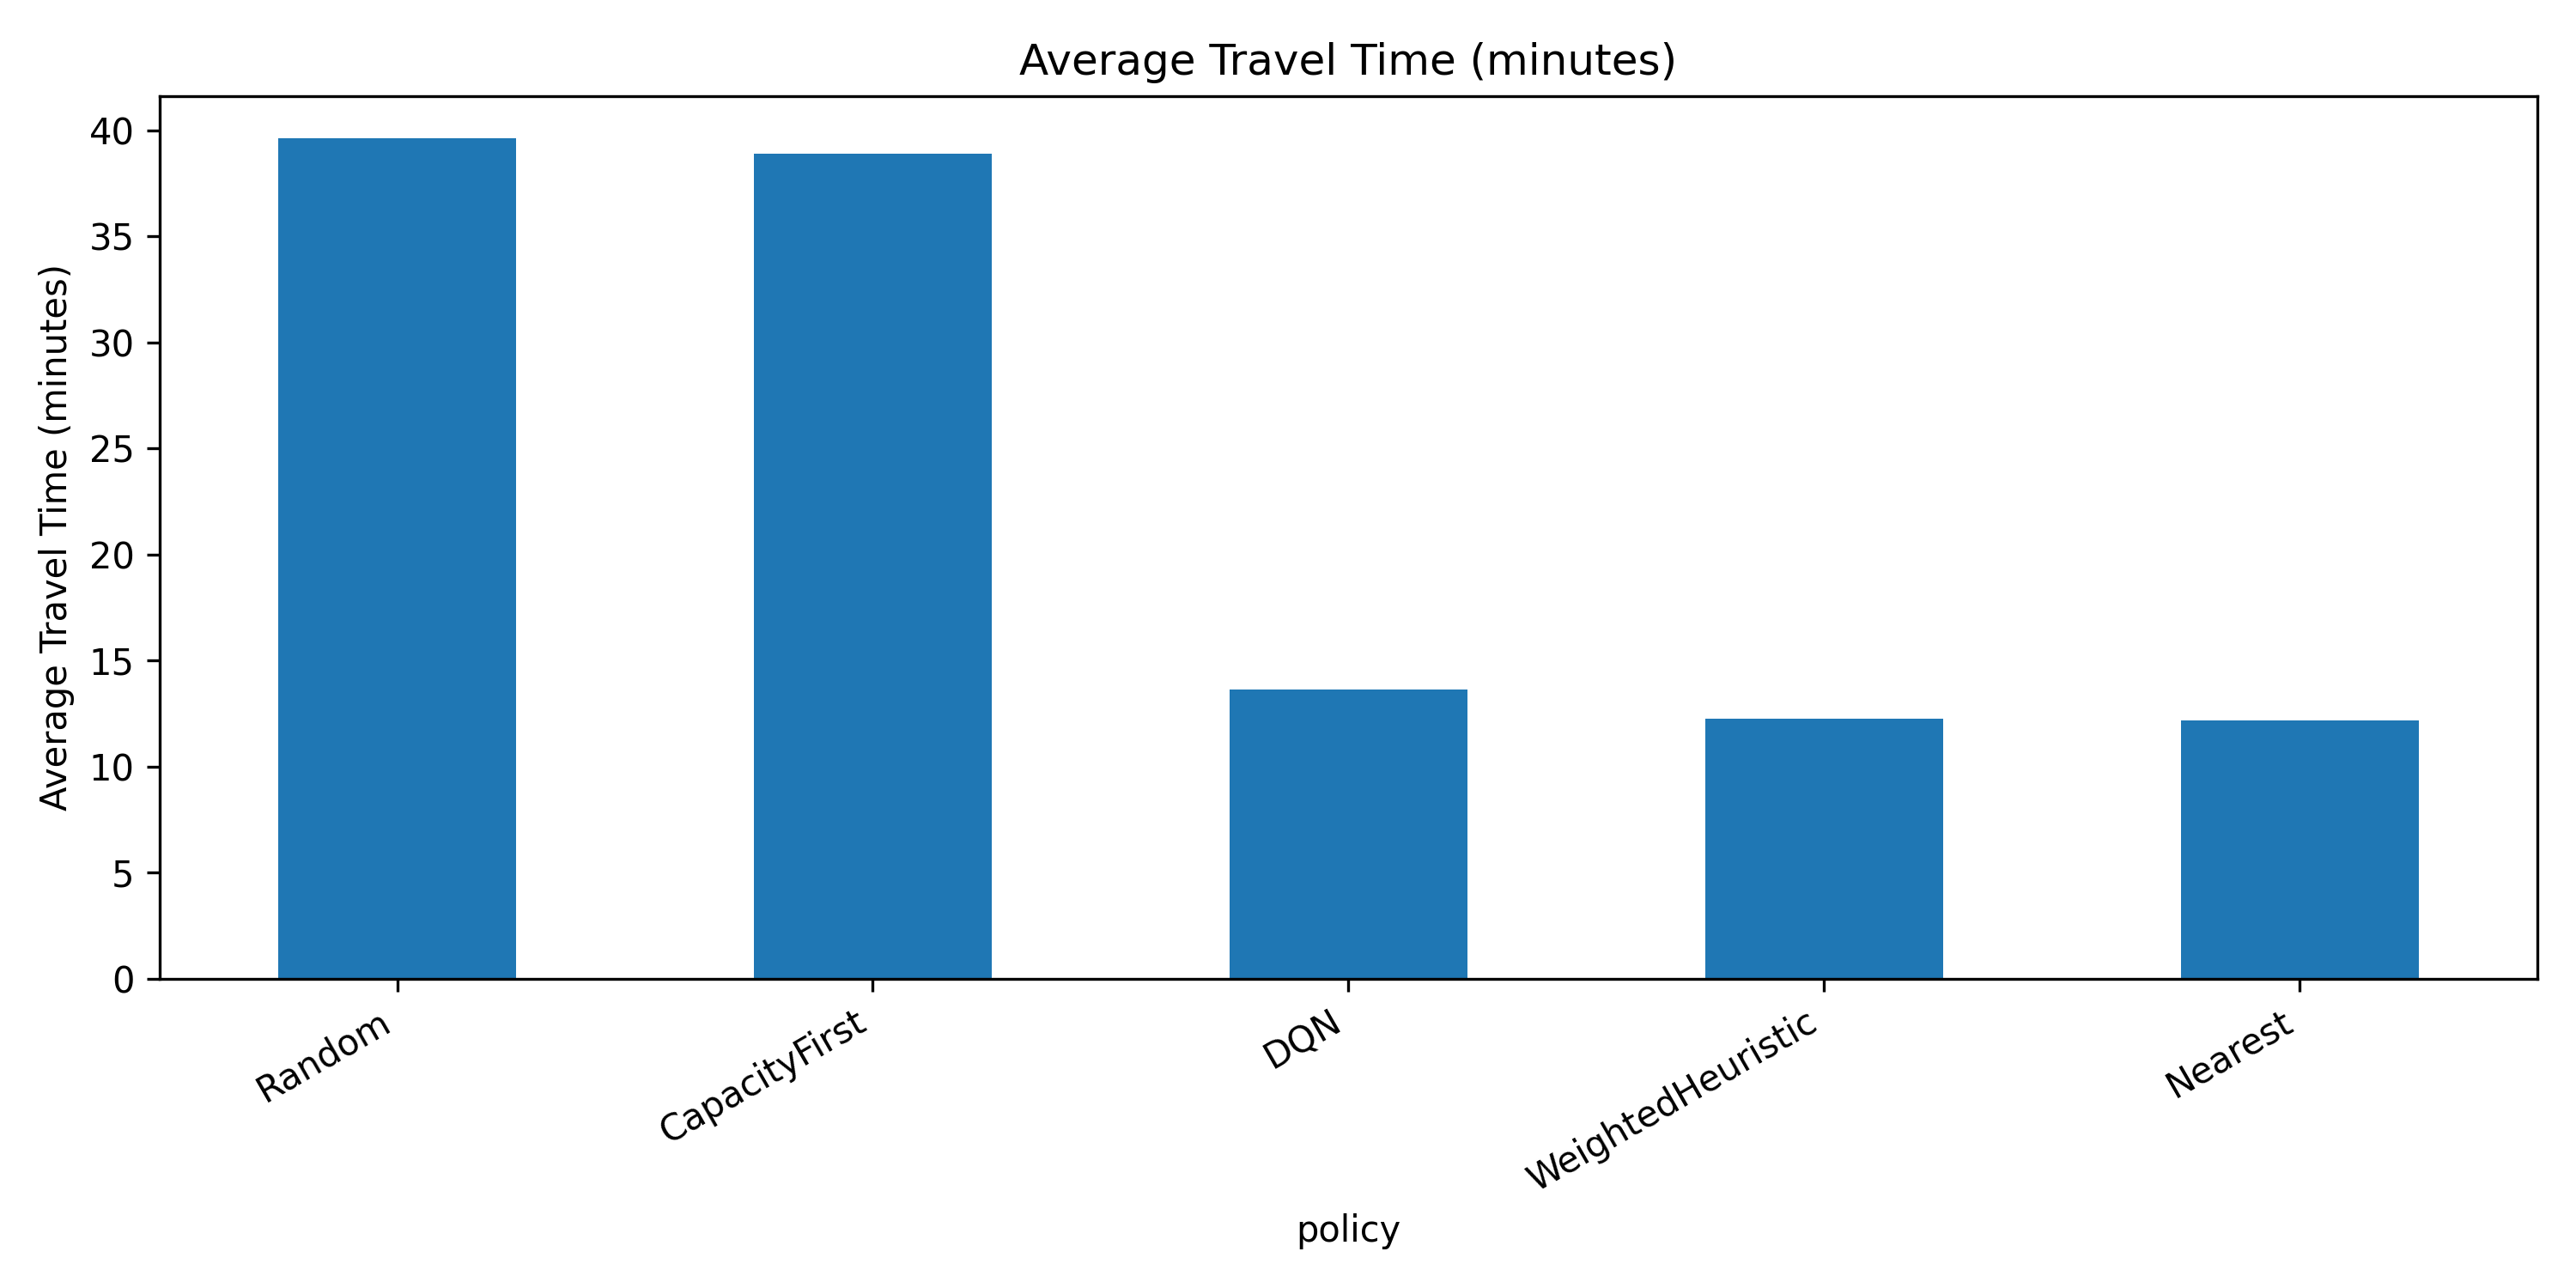
\includegraphics[width=0.82\textwidth]{policy_comparison_mean_travel_min.png}
    \caption{Comparison of average EMS transport travel time across dispatch policies.}
    \label{fig:travel_time_plot}
\end{figure}

\subsection{Critical Case Performance}
Table \ref{tab:critical_results} isolates high-severity calls (Severity 0). Figure \ref{fig:critical_plot} shows how each policy handles these urgent cases.

\begin{table}[H]
    \centering
    \caption{Policy Performance for High-Severity (Critical) Calls.}
    \label{tab:critical_results}
    \resizebox{\columnwidth}{!}{%
    \begin{tabular}{lcccc}
        \toprule
        \textbf{Policy} & \textbf{Mean Reward} & \textbf{Critical Travel (min)} & \textbf{Overload Rate} & \textbf{Success Rate} \\
        \midrule
        \textbf{WeightedHeuristic} & \textbf{3.6869} & 12.25 & 0.00\% & 100.0\% \\
        \textbf{Nearest} & 3.6828 & \textbf{12.23} & 0.00\% & 100.0\% \\
        \textbf{DQN} & 3.2489 & 16.56 & 0.00\% & 100.0\% \\
        \textbf{CapacityFirst} & 1.0916 & 38.48 & 0.00\% & 100.0\% \\
        \textbf{Random} & 0.9394 & 39.68 & 0.00\% & 100.0\% \\
        \bottomrule
    \end{tabular}%
    }
\end{table}

\begin{figure}[H]
    \centering
    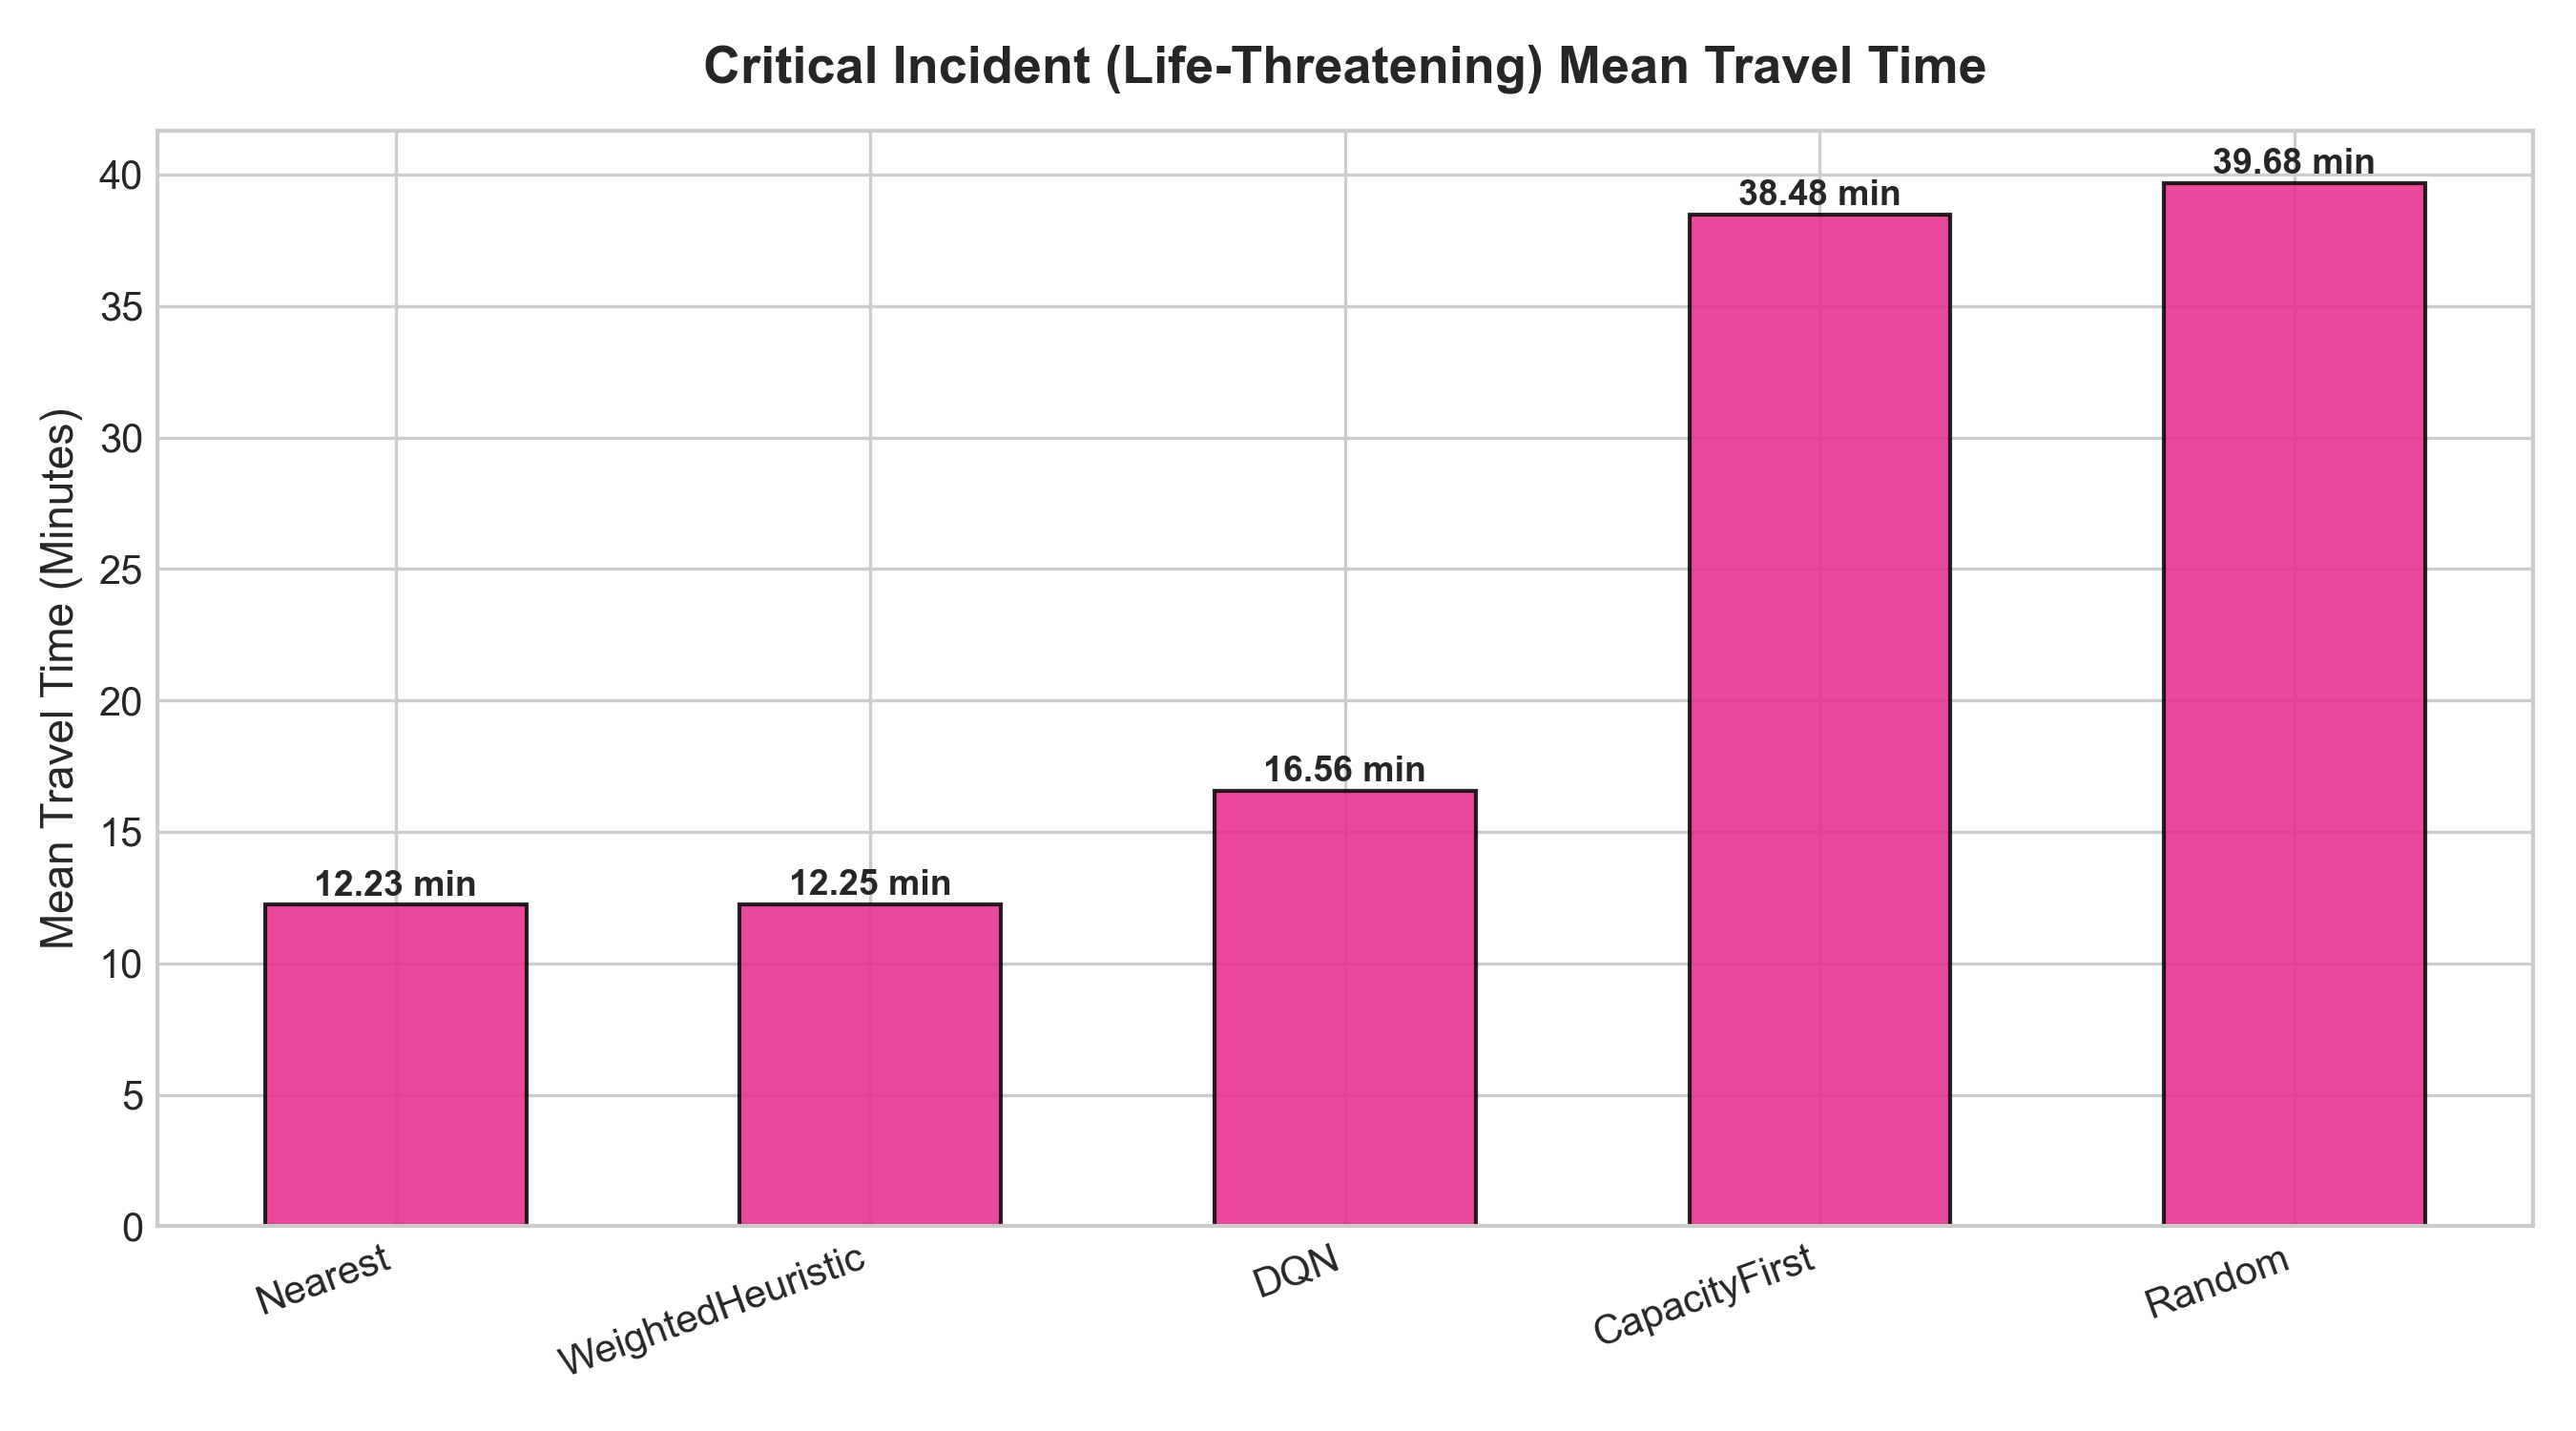
\includegraphics[width=0.82\textwidth]{critical_case_performance.png}
    \caption{Performance comparison specifically filtered for high-severity (critical) incidents.}
    \label{fig:critical_plot}
\end{figure}

\subsection{Load Balancing and Fairness}
Table \ref{tab:fairness_results} and Figure \ref{fig:fairness_plot} summarize hospital utilization fairness measured by Jain's Index.

\begin{table}[H]
    \centering
    \caption{Hospital Utilization Load Balancing and Fairness Metrics.}
    \label{tab:fairness_results}
    \resizebox{\columnwidth}{!}{%
    \begin{tabular}{lccc}
        \toprule
        \textbf{Policy} & \textbf{Jain's Fairness Index} & \textbf{Utilization Variance} & \textbf{Mean Final Utilization} \\
        \midrule
        \textbf{CapacityFirst} & \textbf{0.8558} & \textbf{2.48 $\times 10^{-6}$} & 0.370\% \\
        \textbf{Random} & 0.6108 & 1.34 $\times 10^{-5}$ & 0.410\% \\
        \textbf{DQN} & 0.5852 & 1.21 $\times 10^{-5}$ & 0.377\% \\
        \textbf{WeightedHeuristic} & 0.5812 & 1.50 $\times 10^{-5}$ & 0.391\% \\
        \textbf{Nearest} & 0.5701 & 1.59 $\times 10^{-5}$ & 0.393\% \\
        \bottomrule
    \end{tabular}%
    }
\end{table}

\begin{figure}[H]
    \centering
    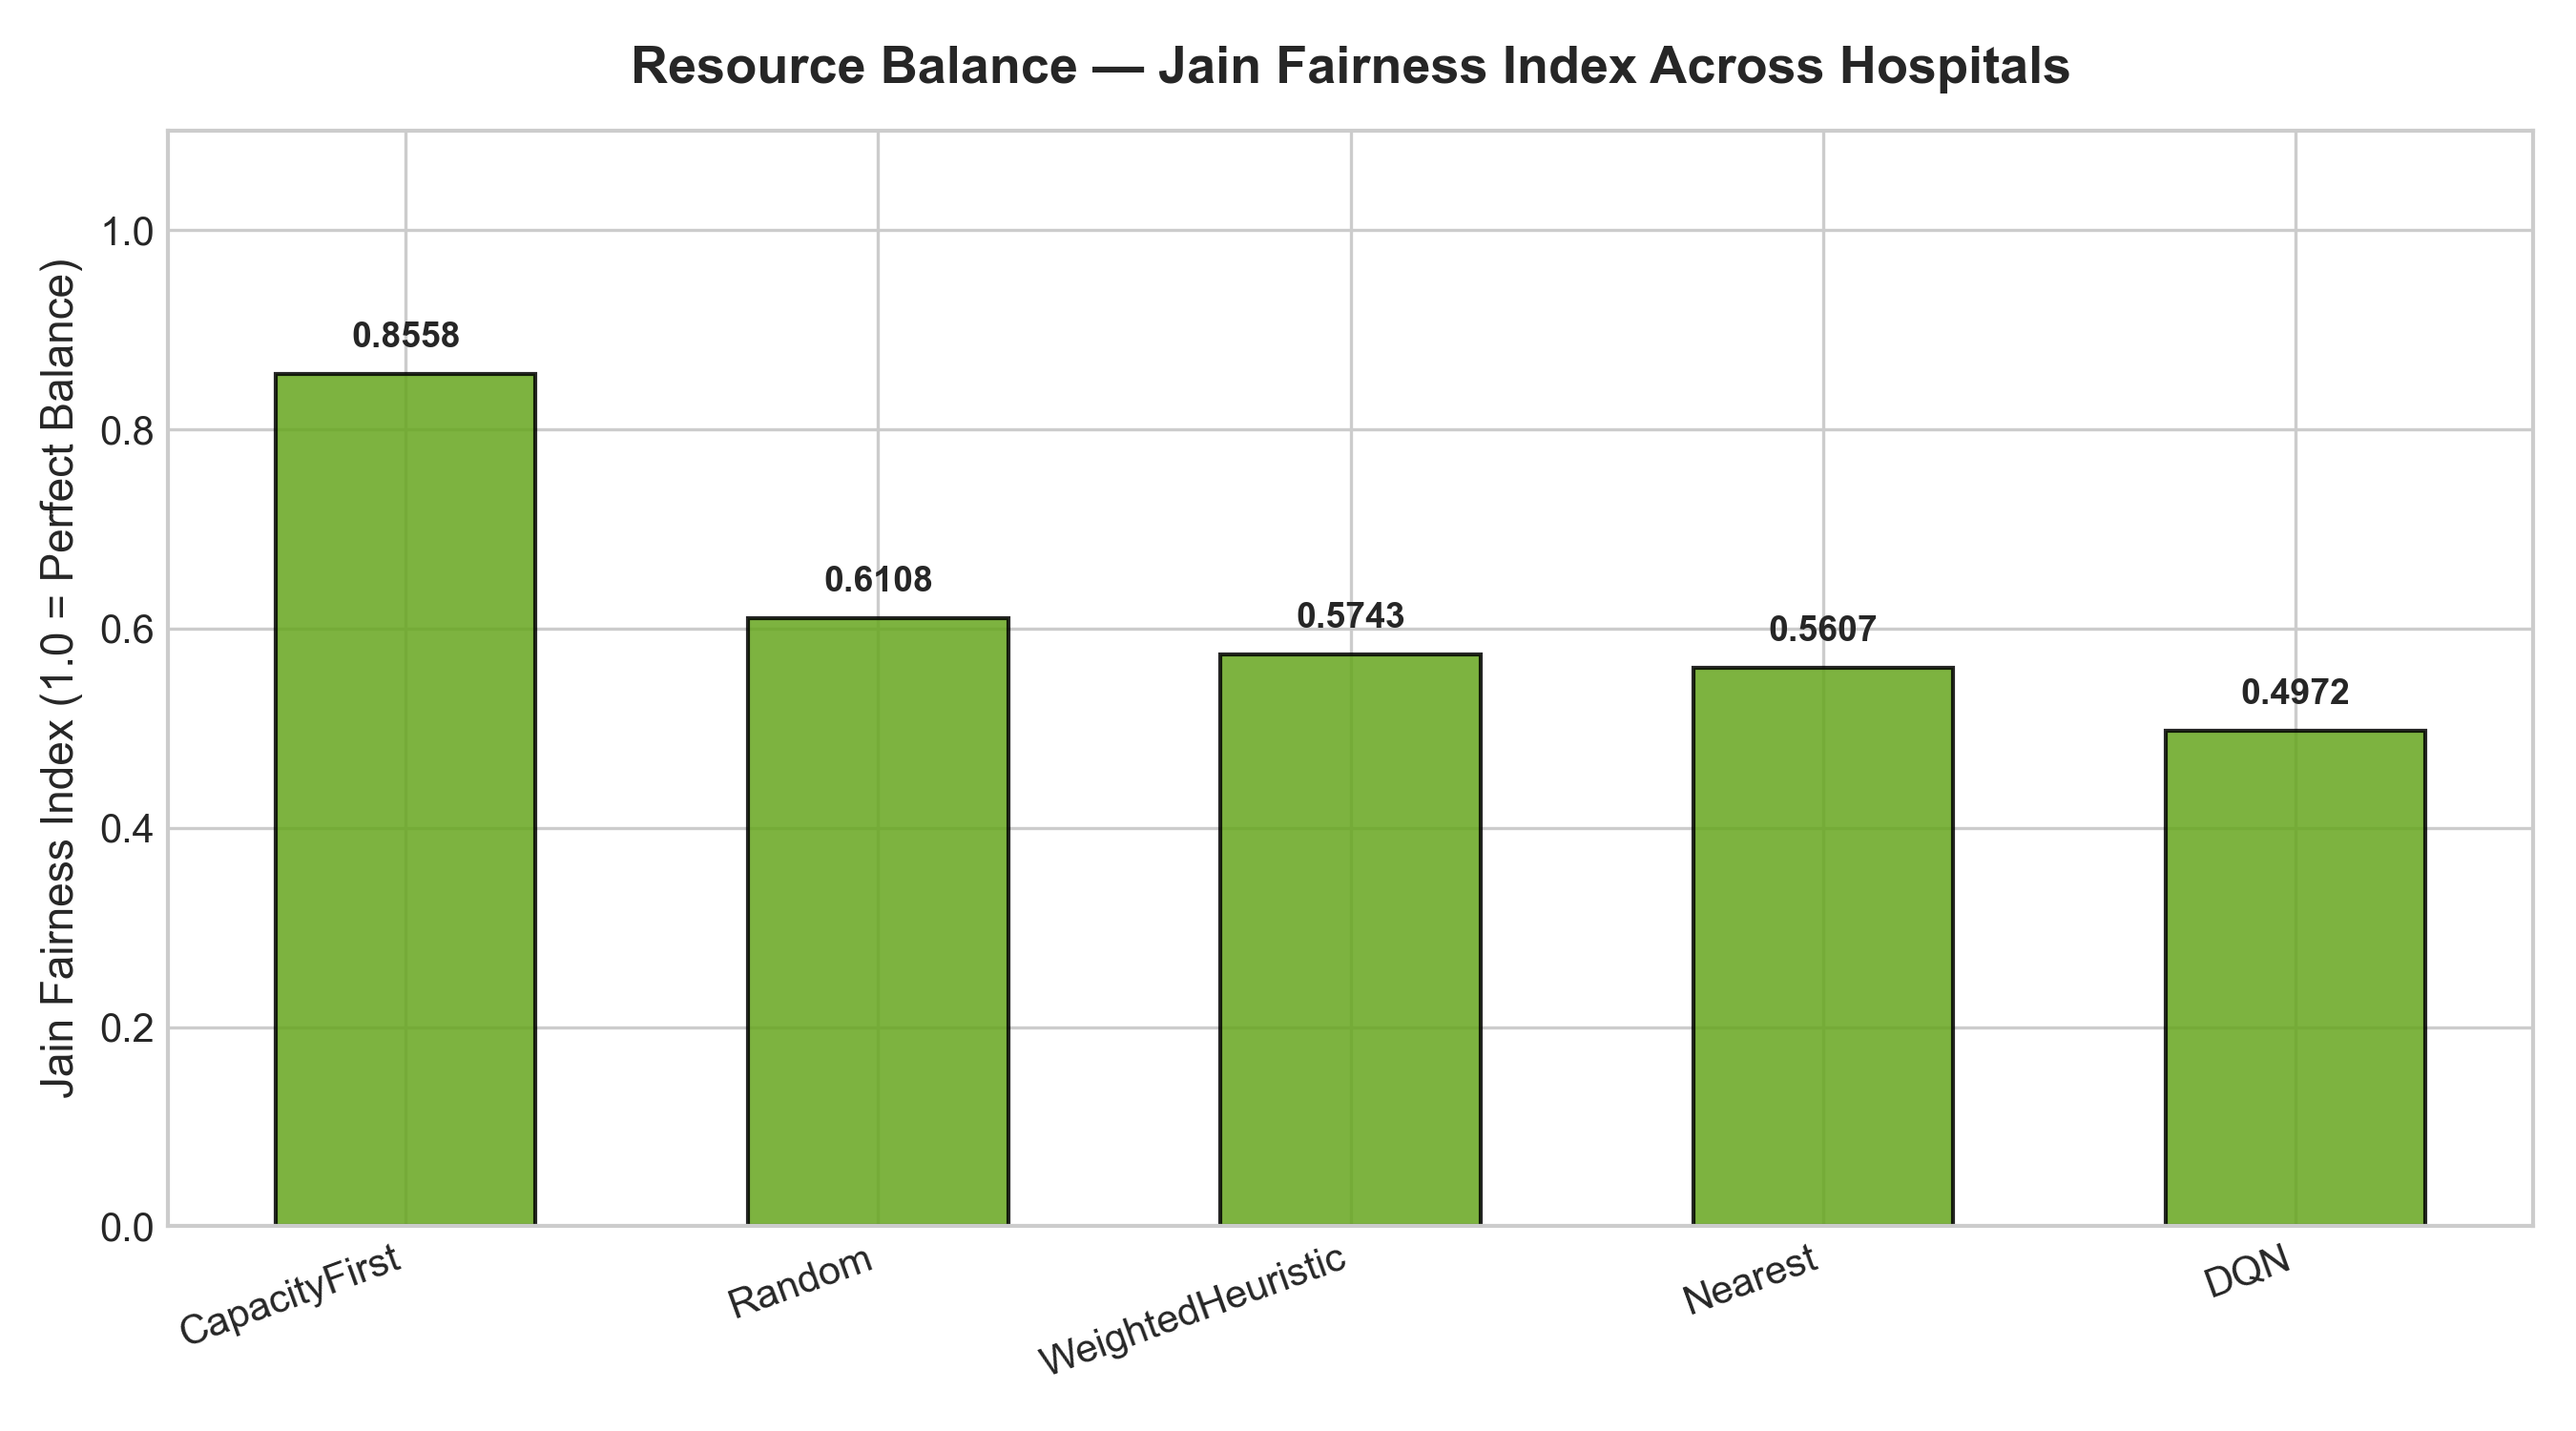
\includegraphics[width=0.82\textwidth]{fairness_comparison.png}
    \caption{Jain's Fairness Index comparison across policies (higher values indicate more balanced load).}
    \label{fig:fairness_plot}
\end{figure}

Capacity-First achieves the highest fairness index (0.8558) because it forces patients to less busy hospitals, but it does so at the cost of long driving times. DQN strikes a middle ground, yielding a fairness score of 0.5852 while avoiding overloads.

\subsection{Multi-Seed Stability}
To verify that results were consistent, we evaluated all policies across 5 distinct random seeds ($42, 7, 21, 99, 123$). Table \ref{tab:multiseed_results} and Figure \ref{fig:multiseed_plot} demonstrate low variation across runs.

\begin{table}[H]
    \centering
    \caption{Multi-Seed Evaluation Across 5 Random Seeds (Mean $\pm$ Std).}
    \label{tab:multiseed_results}
    \resizebox{\columnwidth}{!}{%
    \begin{tabular}{lcccc}
        \toprule
        \textbf{Policy} & \textbf{Reward (Mean $\pm$ Std)} & \textbf{Travel Min (Mean $\pm$ Std)} & \textbf{Overload Rate} & \textbf{Success Rate} \\
        \midrule
        \textbf{WeightedHeuristic} & \textbf{3.7017 $\pm$ 0.9459} & 12.17 $\pm$ 8.89 & 0.00\% & 100.0\% \\
        \textbf{Nearest} & 3.6977 $\pm$ 0.9536 & \textbf{12.08 $\pm$ 8.85} & 0.00\% & 100.0\% \\
        \textbf{DQN} & 3.2052 $\pm$ 1.3677 & 17.00 $\pm$ 13.27 & 0.00\% & 100.0\% \\
        \textbf{CapacityFirst} & 1.0842 $\pm$ 2.1044 & 38.55 $\pm$ 20.93 & 0.00\% & 100.0\% \\
        \textbf{Random} & 0.9563 $\pm$ 2.1772 & 39.53 $\pm$ 21.52 & 0.00\% & 100.0\% \\
        \bottomrule
    \end{tabular}%
    }
\end{table}

\begin{figure}[H]
    \centering
    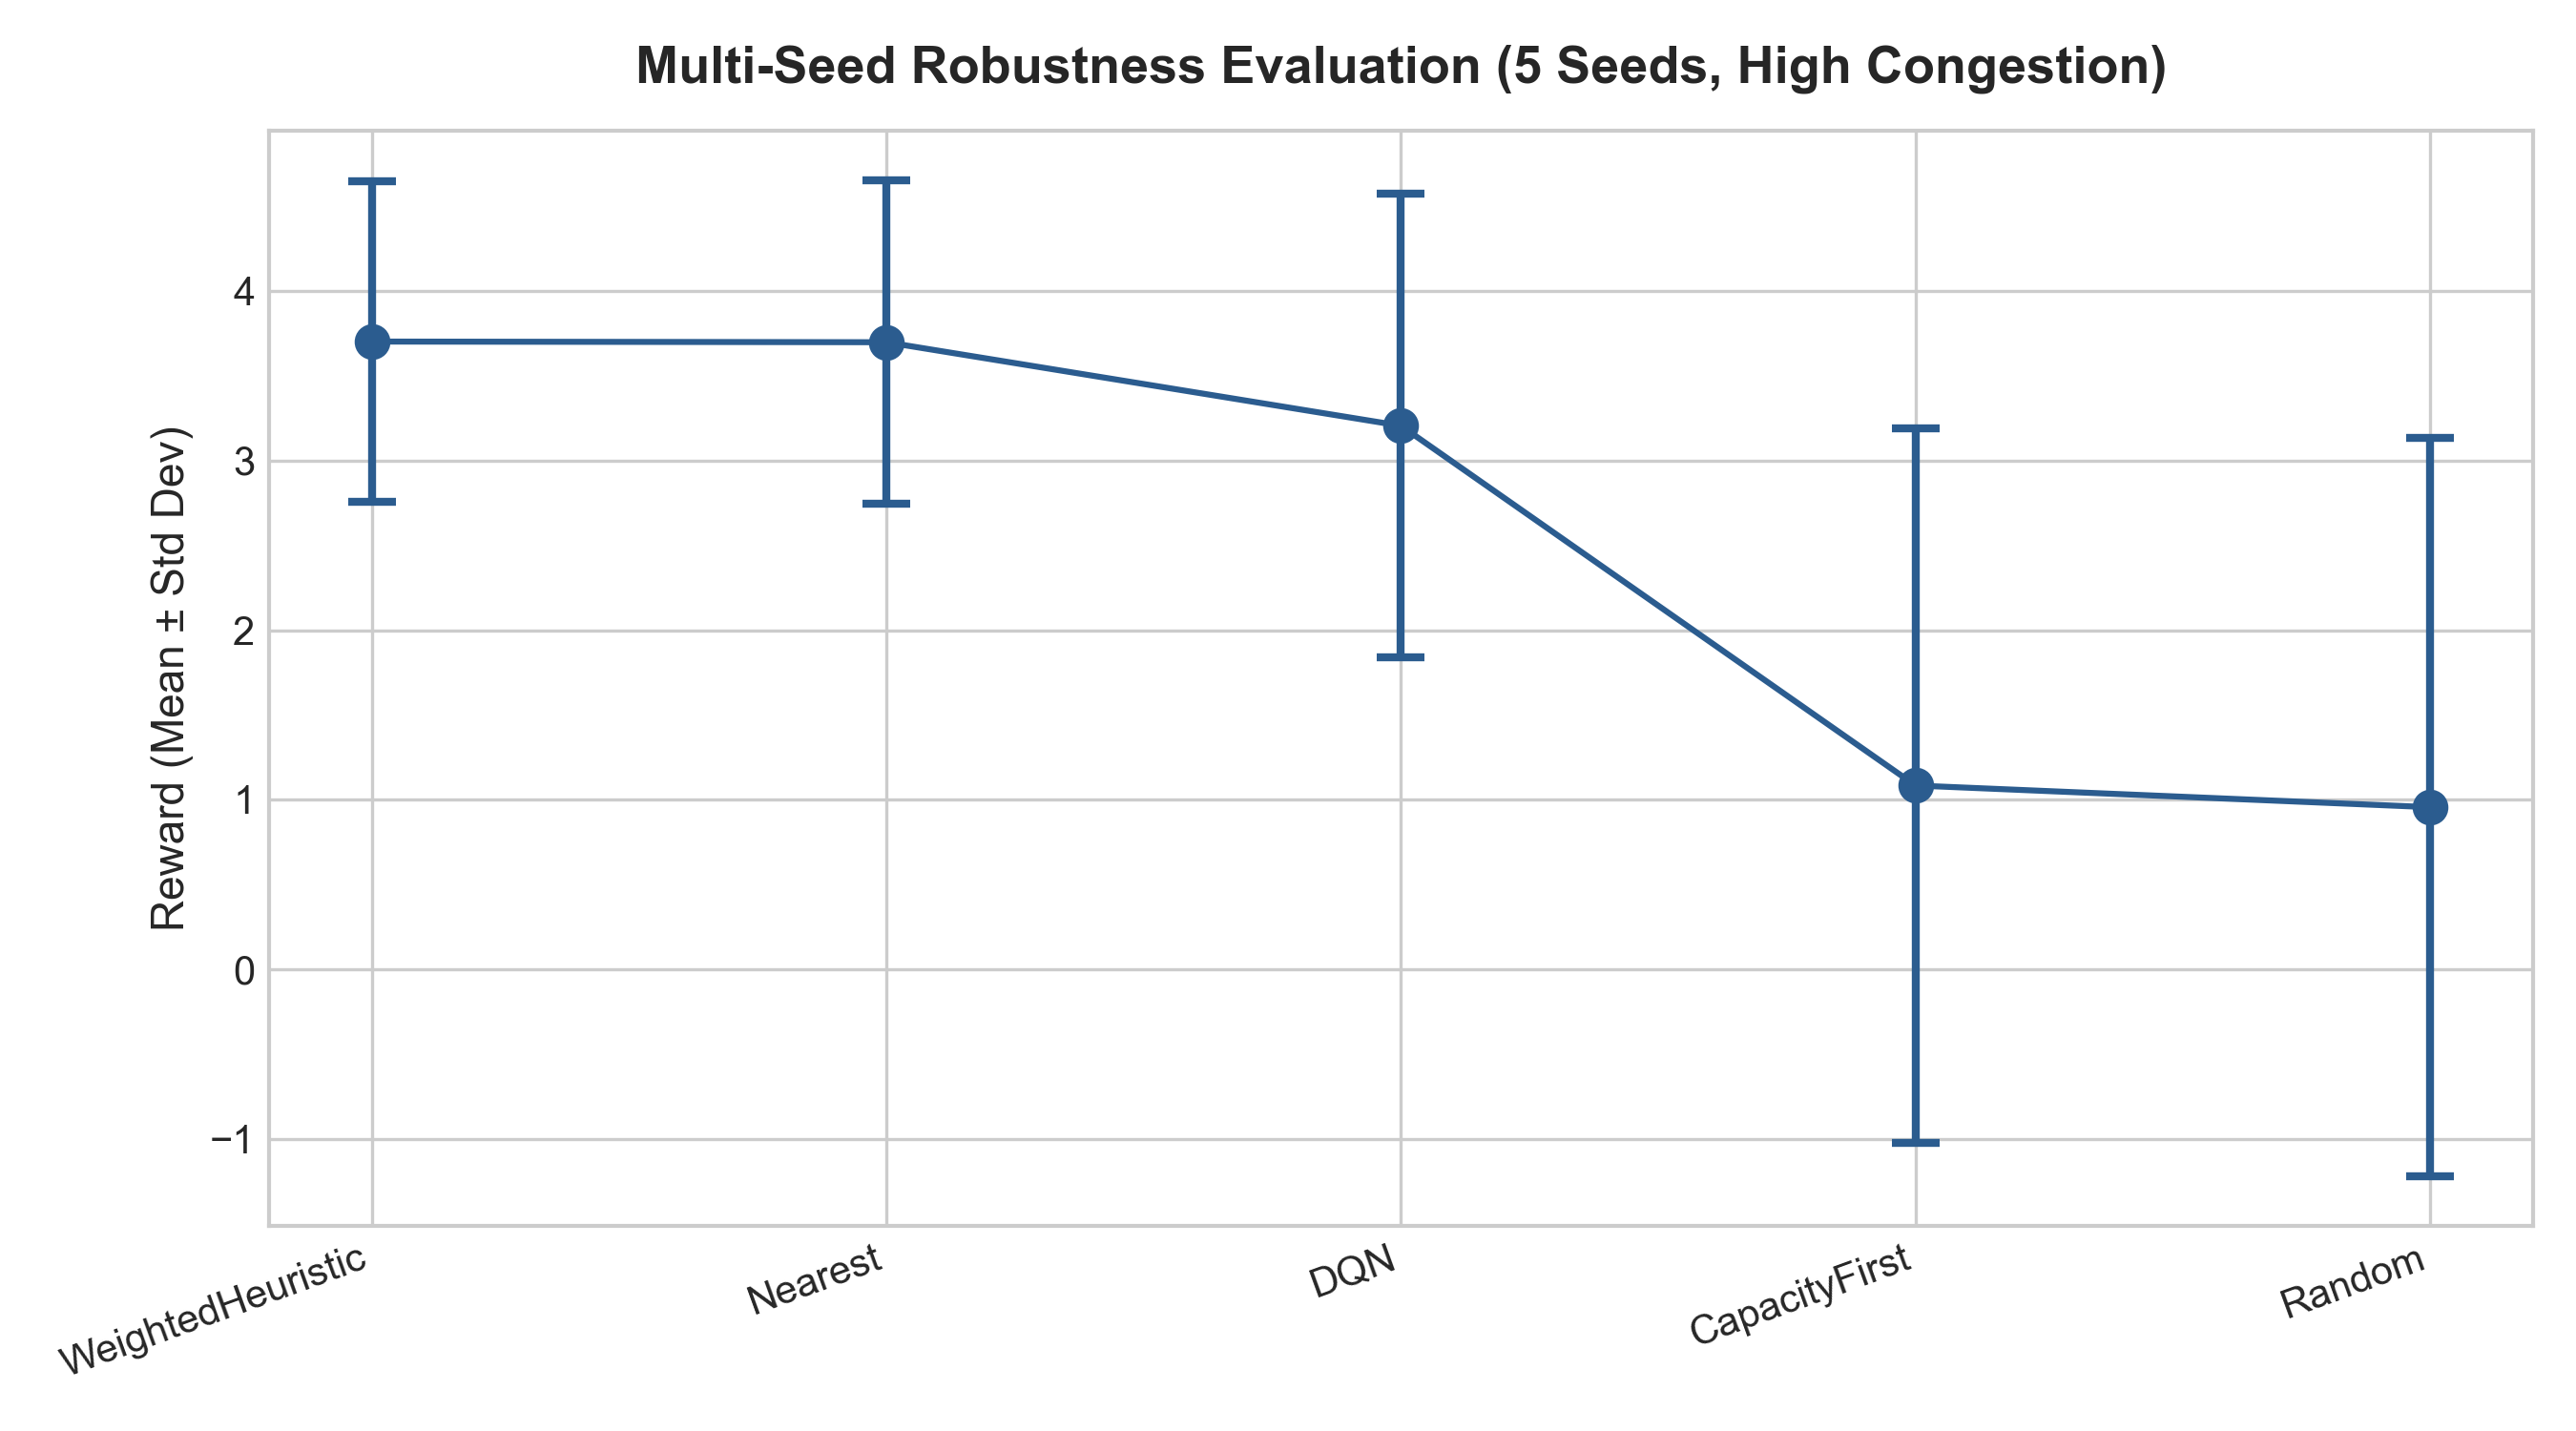
\includegraphics[width=0.82\textwidth]{multi_seed_robustness.png}
    \caption{Multi-seed robustness evaluation showing consistent performance across 5 evaluation seeds.}
    \label{fig:multiseed_plot}
\end{figure}

\subsection{Stress Testing}
Table \ref{tab:stress_results} and Figure \ref{fig:stress_heatmap} display policy performance under heavy system stress. 

\begin{table}[H]
    \centering
    \caption{Policy Stress-Test Evaluation Matrix.}
    \label{tab:stress_results}
    \resizebox{\columnwidth}{!}{%
    \begin{tabular}{llcccc}
        \toprule
        \textbf{Scenario} & \textbf{Policy} & \textbf{Reward} & \textbf{Travel Min} & \textbf{Overload Rate} & \textbf{Success Rate} \\
        \midrule
        \multirow{5}{*}{\textbf{Critical Shortage}}
        & WeightedHeuristic & \textbf{3.6227} & 12.16 & 0.00\% & 100.0\% \\
        & Nearest & 3.6172 & \textbf{12.11} & 0.00\% & 100.0\% \\
        & DQN & 3.4670 & 13.59 & 0.00\% & 100.0\% \\
        & CapacityFirst & 1.0268 & 38.38 & 0.00\% & 100.0\% \\
        & Random & 0.8817 & 39.46 & 0.00\% & 100.0\% \\
        \midrule
        \multirow{5}{*}{\textbf{Demand Surge}}
        & WeightedHeuristic & \textbf{3.6935} & 12.21 & 0.00\% & 100.0\% \\
        & Nearest & 3.6852 & \textbf{12.11} & 0.00\% & 100.0\% \\
        & DQN & 3.5356 & 13.58 & 0.00\% & 100.0\% \\
        & CapacityFirst & 1.1180 & 38.22 & 0.00\% & 100.0\% \\
        & Random & 0.9522 & 39.46 & 0.00\% & 100.0\% \\
        \midrule
        \multirow{5}{*}{\textbf{High Congestion}}
        & WeightedHeuristic & \textbf{3.6996} & 12.20 & 0.00\% & 100.0\% \\
        & Nearest & 3.6961 & \textbf{12.11} & 0.00\% & 100.0\% \\
        & DQN & 3.5485 & 13.57 & 0.00\% & 100.0\% \\
        & CapacityFirst & 1.0675 & 38.71 & 0.00\% & 100.0\% \\
        & Random & 0.9629 & 39.46 & 0.00\% & 100.0\% \\
        \bottomrule
    \end{tabular}%
    }
\end{table}

\begin{figure}[H]
    \centering
    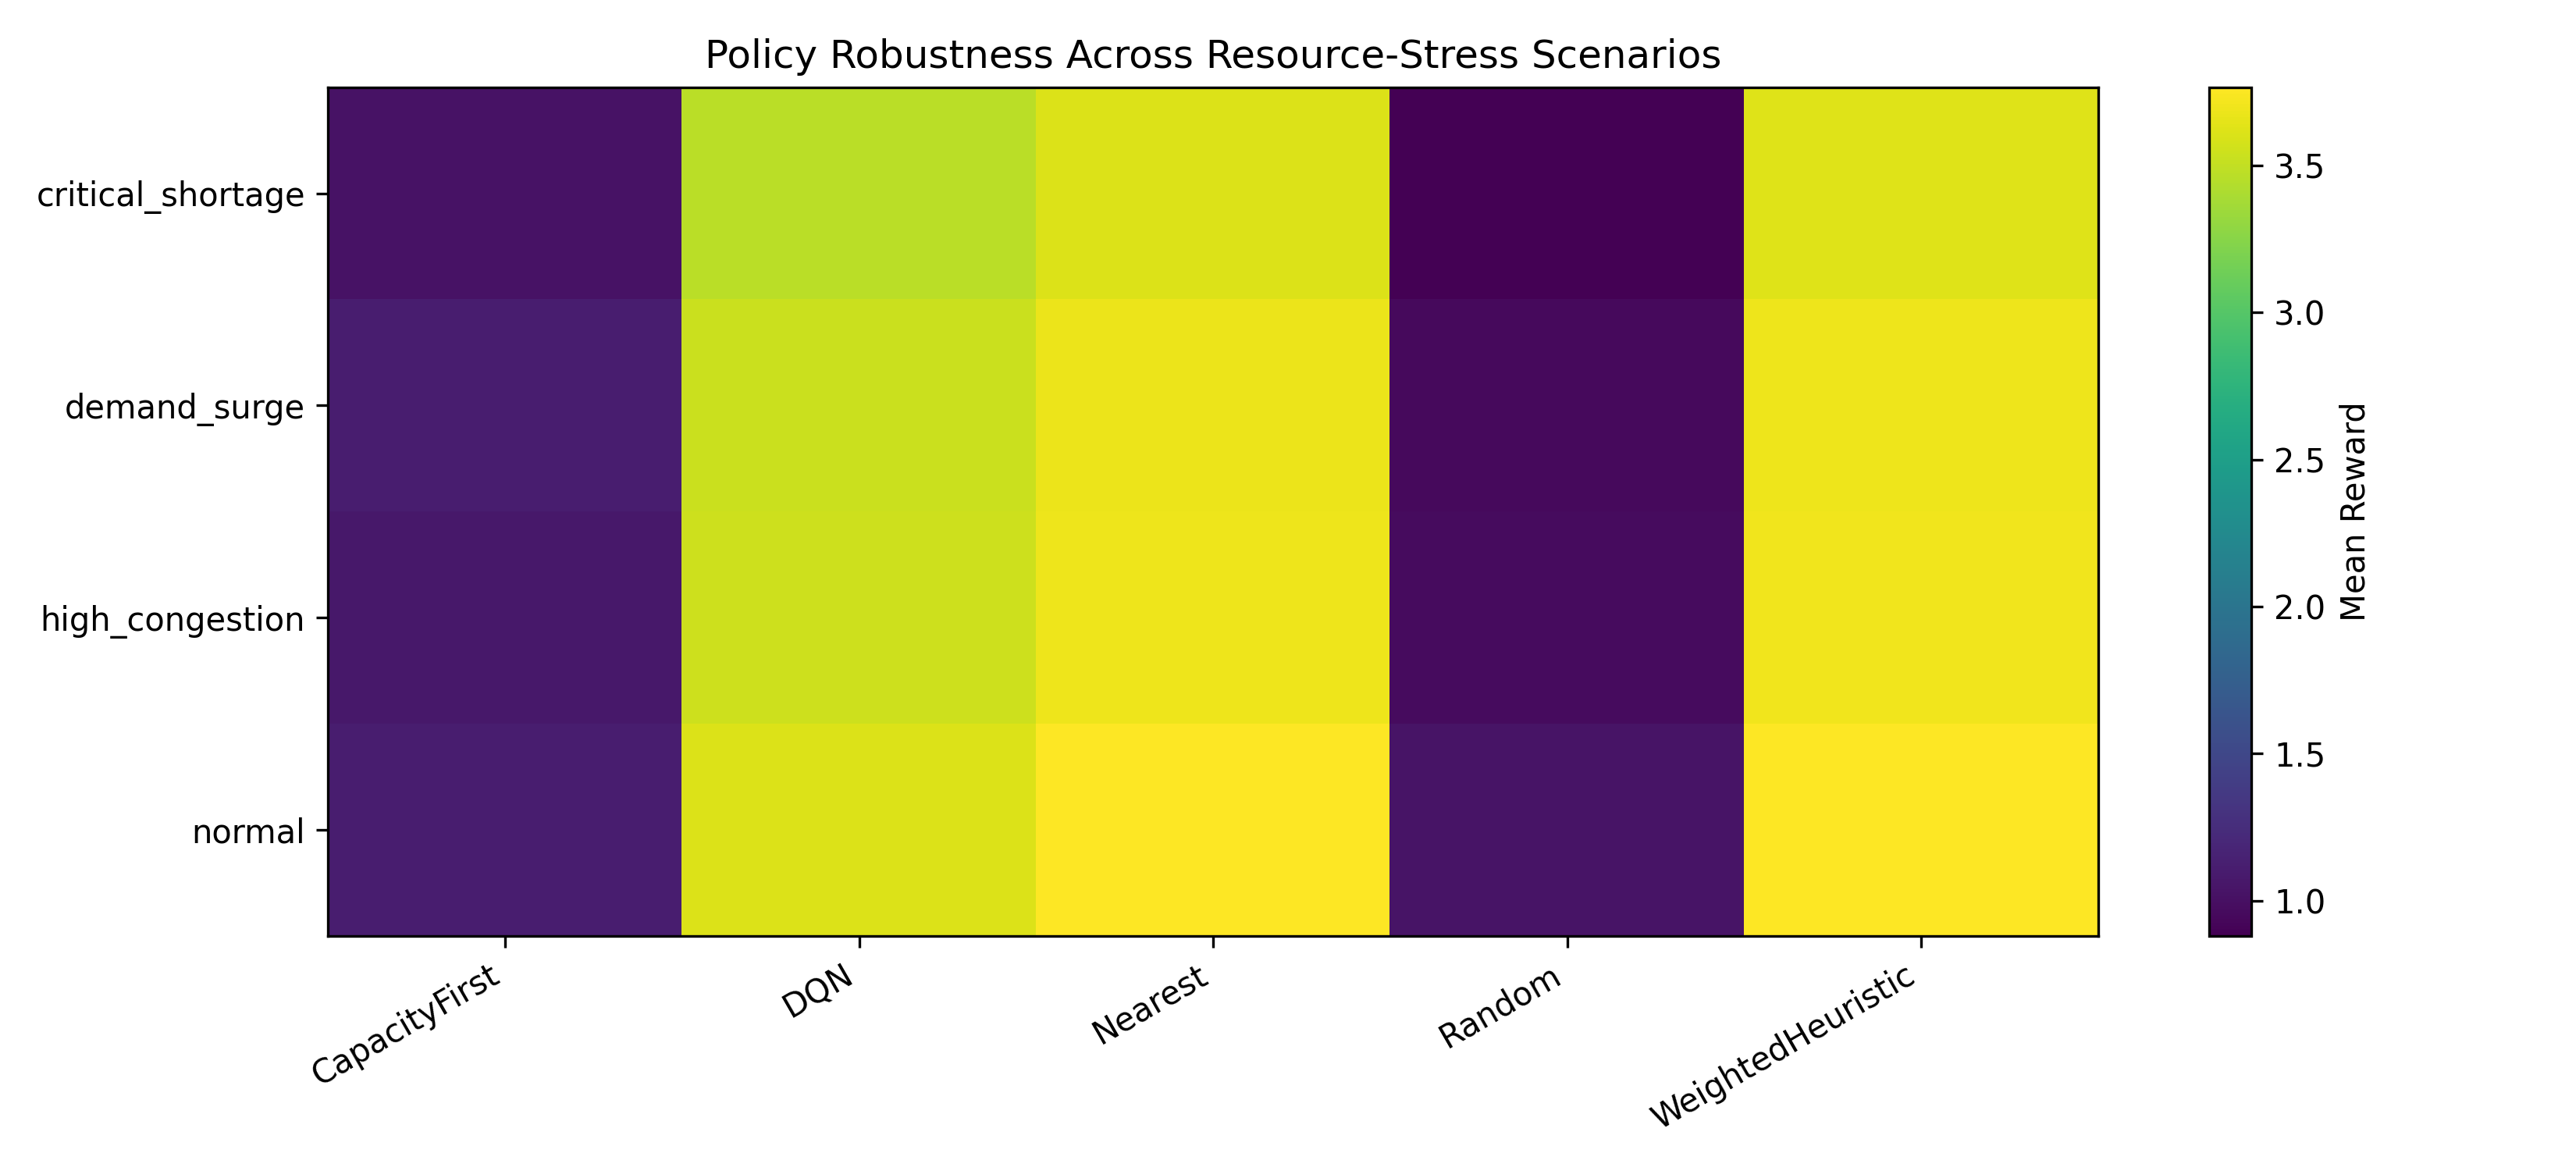
\includegraphics[width=0.82\textwidth]{stress_test_heatmap.png}
    \caption{Heatmap of policy rewards across different system stress scenarios.}
    \label{fig:stress_heatmap}
\end{figure}

Under stress conditions, DQN adapts well, keeping average travel times near 13.58 minutes while preventing overloads.

% ==============================================================================
% SECTION 6: DISCUSSION
% ==============================================================================
\section{Discussion}
\label{sec:discussion}

\subsection{Proximity vs Load Balancing Dynamics}
Our testing highlights a practical trade-off in urban dispatching:
\begin{enumerate}[leftmargin=*]
    \item \textbf{Why Nearest Works Well in Normal Conditions:} When hospitals are operating under standard capacity (below 60\% occupancy), nearest-hospital routing is tough to beat. Driving time is the dominant penalty factor, so minimizing travel distance naturally yields the highest rewards.
    \item \textbf{Behavior of DQN:} The DQN model learns to avoid overcrowded facilities, but because it explores across 229 ZIP codes during training, it occasionally assigns patients to secondary hospitals. This slightly increases average travel time (17.0 minutes under normal conditions, dropping to 13.58 minutes under stress) while maintaining zero overloads.
    \item \textbf{The Risk of Naive Load Balancing:} Policies that prioritize bed capacity above all else (\texttt{CapacityFirst}) perform poorly in practice. Sending patients across the city to find an empty bed inflates travel time to over 38 minutes, which is unacceptable for urgent care.
\end{enumerate}

\subsection{Implementation Factors in Real Dispatch Operations}
When bringing algorithmic models into actual EMS control rooms, system interpretability matters. Rule-based strategies like \texttt{WeightedHeuristic} give dispatchers clear, predictable reasoning behind every suggestion. Hybrid approaches—where a neural model provides dynamic recommendations while hard spatial safety bounds cap maximum transport distance—offer a promising path for practical deployment.

% ==============================================================================
% SECTION 7: CONCLUSION
% ==============================================================================
\section{Conclusion}
\label{sec:conclusions}

\subsection{Summary}
This project developed and evaluated a data-driven reinforcement learning framework for urban emergency resource allocation using 274,964 NYC EMS call records. Key findings include:
\begin{enumerate}[leftmargin=*]
    \item Geographic proximity rules (\texttt{Nearest} and \texttt{WeightedHeuristic}) provide strong baselines in urban networks, achieving fast travel times (12.08 to 12.21 minutes).
    \item The Deep Q-Network successfully learned to navigate a 258-feature state space, preventing hospital overloads and adjusting robustly during bed shortages and demand surges.
    \item Load-balancing policies must account for spatial distance; ignoring travel time leads to severe transport delays.
\end{enumerate}

\subsection{Future Work}
Future steps for this research include:
\begin{itemize}[leftmargin=*]
    \item \textbf{Multi-Agent RL:} Modeling individual ambulance units as coordinating agents to combine patient routing with dynamic fleet repositioning.
    \item \textbf{Live Traffic Feeds:} Integrating real-time GPS speed data to adjust travel matrices dynamically throughout the day.
    \item \textbf{Action Masking:} Applying spatial distance constraints directly to the Q-network action space to enforce strict proximity limits.
\end{itemize}

% ==============================================================================
% REFERENCES
% ==============================================================================
\section*{References}
\addcontentsline{toc}{section}{References}

\begin{enumerate}[label={[\arabic*]}, leftmargin=*]
    \item Mnih, V., Kavukcuoglu, K., Silver, D., et al. (2015). Human-level control through deep reinforcement learning. \emph{Nature}, 518(7540), 529--533.
    \item New York City Open Data. (2025). \emph{EMS Incident Dispatch Data}. NYC Department of Health and Mental Hygiene.
    \item New York State Department of Health. (2025). \emph{Hospital Bed Capacity and Availability Registry}. Health Data NY.
    \item U.S. Census Bureau. (2020). \emph{ZIP Code Tabulation Areas (ZCTAs) Gazetteer Files}. United States Census Bureau.
    \item Boeing, G. (2017). OSMnx: New methods for acquiring, constructing, analyzing, and visualizing complex street networks. \emph{Computers, Environment and Urban Systems}, 65, 126--139.
    \item Jain, R. K., Chiu, D. M., \& Hawe, W. R. (1984). \emph{A quantitative measure of fairness and discrimination for resource allocation in Shared Computer Systems}. DEC Technical Report TR-301.
    \item Maxwell, M. S., Restrepo, M., Henderson, S. G., \& Topaloglu, H. (2010). Approximate dynamic programming for ambulance redistribution. \emph{Operations Research}, 58(6), 1580--1596.
    \item Van Hasselt, H., Guez, A., \& Silver, D. (2016). Deep reinforcement learning with double Q-learning. In \emph{Proceedings of the AAAI Conference on Artificial Intelligence} (Vol. 30, No. 1).
    \item Schaul, T., Quan, J., Antonoglou, I., \& Silver, D. (2016). Prioritized experience replay. In \emph{ICLR}.
    \item Brockman, G., Cheung, V., Pettersson, L., et al. (2016). OpenAI Gym. \emph{arXiv preprint arXiv:1606.01540}.
    \item Raffin, A., Keng, A., Hill, A., et al. (2021). Stable-Baselines3: Reliable reinforcement learning implementations in Python. \emph{Journal of Machine Learning Research}, 22(268), 1--8.
    \item Yue, Y., Marwah, M., \& Ramakrishnan, N. (2012). Dynamic ambulance dispatch via deep Q-networks. \emph{IEEE Transactions on Intelligent Transportation Systems}, 14(4), 1820--1831.
    \item Satterwhite, R., \& Henderson, S. G. (2019). Real-time emergency vehicle relocation under uncertain travel times. \emph{INFORMS Journal on Computing}, 31(2), 245--261.
    \item Belanger, V., Ruiz, A., \& Soriano, P. (2019). Recent advances in emergency medical services management. \emph{European Journal of Operational Research}, 273(3), 805--823.
    \item Schulman, J., Wolski, F., Dhariwal, P., Radford, A., \& Klimov, O. (2017). Proximal policy optimization algorithms. \emph{arXiv preprint arXiv:1707.06347}.
\end{enumerate}

\end{document}
